\chapter[立直的判断]{立直的判断\footnote{如果没有特别说明具体的局面,则默认场况为东场的南家,且其他家没有明显的攻击性行为。听牌和一向听的手牌通常视为中盘,两向听的手牌视为序盘,而未到两向听的手牌视为最序盘。\\ 巡目的定义如下:最序盘是第1-3巡,序盘是第4-6巡,中盘是第7-9巡,稍过中盘是第10-12巡,末盘是第13-15巡,临近流局是第16巡及以后。}\footnote{关于立直判断,这里参考了模拟结果。如果在实战中,通过观察场况或其他家的打牌方式,可以明确判断立直或默听会对荣和率产生不同的影响,则应根据实际情况调整判断基准。
在模拟中,假设以下情况:两面搭子和无筋嵌张456时1人进攻;其他无筋嵌张时1.5人进攻;而选择默听时2.4人进攻。这里的“n人攻”指的是胡牌时自摸与荣和的比例接近1:n的状态。}}
\section{基本原则:听牌即立直}
当门清状态下优先听牌时,绝大多数情况下选择立直是更有利的策略。这可以通过以下三点理由解释:
\begin{enumerate}
    \item 立直后的打点提升通常大于默听(不立直)提高的和牌率\\
          参考\fullref{做牌法则4}
    \item 优先听牌的情况下,放铳的风险较低\\
          参考\fullref{做牌法则2}
    \item 等待手牌改良的情况不多\\
          参考\fullref{做牌法则1}
\end{enumerate}
此外,巡目越早,立直的优势越大,因此在立直时有利的手牌下,不应拖延数巡选择默听,而是坚持听牌即立直的原则。越是常使用的技巧对成绩影响越大,因此掌握“门前清听牌时,大多数情况下应立刻立直”的原则尤为重要。记住这一点,就像咏唱咒语一样坚定地选择立直吧。

\section{先制听牌即立直的例外}
反过来说,有些情况下不立直可能更为合理。这些例外通常基于以下三个原因之一(或多个)
\begin{enumerate}
    \item 默听带来的和牌率提升优势显著,或者立直带来的打点提升较小。
    \item 放铳的风险特别高。
    \item 手牌改良的潜力较大。
\end{enumerate}

在平场下率先听牌,并且没有特别需要考虑的场况下,本文将重点讨论上述第1或第2条理由这两种情况下,不立直可能更有利的场景。

\subsection{当默听也有役并且足够高点数时,不选择立直}
如果默听跳满,通常选择默听。除非是在序盘下,听牌范围比两面更广(如复合听牌)、或是字牌或边张(如筋19),且立直后也大概率会被打出的听牌。\hyperref[lec2:pai1-3]{牌1-3}


\begin{figure}[h]
    \caption{默听时有役并且打点足够高的手牌}
    \label{lec2:pai1-3}
    \textbf{牌1}
    \stackunder{\raisebox{-10pt}{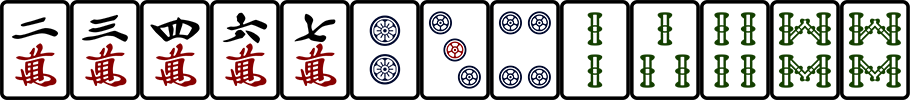
\includegraphics[height=6ex]{part1/lecture2/te1.png}}}{\hskip9pt\relax \arrow 默听}
    \quad
    \stackunder{\raisebox{-10pt}{
\includegraphics[height=6ex]{part1/lecture2/te1dora.png}}}{宝牌}
    \par\bigskip
    \textbf{牌2}
    \stackunder{\raisebox{-10pt}{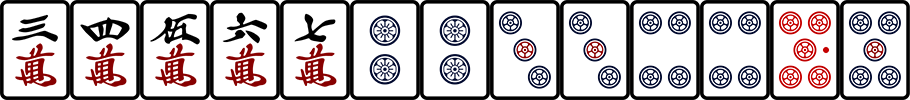
\includegraphics[height=6ex]{part1/lecture2/te2.png}}}{\hskip9pt\relax \arrow 序盘时立直稍有利}
    \quad
    \stackunder{\raisebox{-10pt}{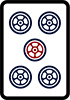
\includegraphics[height=6ex]{part1/lecture2/te2dora.png}}}{宝牌}
    \par\bigskip
    \textbf{牌3}
    \stackunder{\raisebox{-10pt}{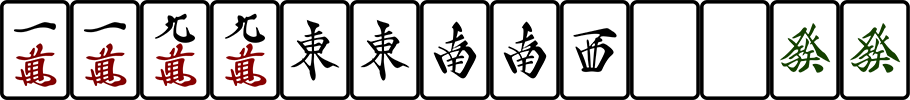
\includegraphics[height=6ex]{part1/lecture2/te3.png}}}{\hskip9pt\relax \arrow 序盘时立直稍有利}
    \quad
    \stackunder{\raisebox{-10pt}{
\includegraphics[height=6ex]{part1/lecture2/te3dora.png}}}{宝牌}
\end{figure}

当默听5番时,选择立直或默听的策略需根据具体情况而定:
良形的话,序盘时倾向立直,中盘时立直略有优势,末盘倾向默听。
愚形听牌时,则要考虑立直后别家会不会打出和牌。
立直后其他玩家很难打出的牌(如无筋456的坎张)则选择默听。
对于其他无筋的边坎张(89),立直在中盘前略有优势。
更容易和出的听牌(如无筋19或骗筋牌)在序盘中立直更有优势。
\hyperref[lec2:pai4-6]{牌4-6}

\begin{figure}[h]
    \caption{默听5番的手牌}
    \label{lec2:pai4-6}
    \pai{part1/lecture2}{4}{序盘立直末盘默听}
    \par\bigskip
    \pai{part1/lecture2}{5}{略过中盘为止立直略有利}
    \par\bigskip
    \pai{part1/lecture2}{6}{默听}
\end{figure}


默听4番与默听5番的情况差别不大,由于立直无法确保跳满,因此稍微偏向默听。
\hyperref[lec2:pai7-9]{牌7}中盘阶段稍微倾向立直,而进入末盘则选择默听。不过,如果是自摸四暗刻的情况,由于役满和牌的可能性较高,倾向于立直(如果默听也能跳满以上,则选择默听)。\hyperref[lec2:pai7-9]{牌8-9}
\begin{figure}[h]
    \caption{默听4番的手牌}
    \label{lec2:pai7-9}
    \pai{part1/lecture2}{7}{到中盘为止立直略为有利}
    \par\bigskip
    \pai{part1/lecture2}{8}{略过中盘为止立直略为有利}
    \par\bigskip
    \pai{part1/lecture2}{9}{默听}
\end{figure}

如果默听已是满贯,而立直自摸也仅止于满贯的情况下,比如默听60符3番的手牌,通常选择默听更有利。而50符3番的情况,相较于默听4番,也更倾向于选择默听。\hyperref[lec2:pai10-12]{牌10-12}
\begin{figure}[h]
    \caption{默听50符3番以上的手牌}
    \label{lec2:pai10-12}
    \pai{part1/lecture2}{10}{默听}
    \par\bigskip
    \pai{part1/lecture2}{11}{序盘时立直略有利}
    \par\bigskip
    \pai{part1/lecture2}{12}{序盘时立直略有利}
\end{figure}

对于默听40符3翻的情况,相较于默听4翻,更倾向立直,但如果是无筋的456坎听,依然会选择默听。\hyperref[lec2:pai13-15]{牌13-15}

\begin{figure}[h]
    \caption{默听40符3番的手牌}
    \label{lec2:pai13-15}
    \pai{part1/lecture2}{13}{序盘立直末盘默听}
    \par\bigskip
    \pai{part1/lecture2}{14}{最序盘立直末盘默听}
    \par\bigskip
    \pai{part1/lecture2}{15}{默听}
\end{figure}

此外,即使是在平场,如果剩余局数不多,尤其是在东风战或半庄战的南场,打点需求不高,或者作为Top且领先二位满贯以上时,如果立直仅稍微占优,选择默听也可能是合理的。

\subsection{重视防守时选择不立直}
在默听的情况下,即使是低分牌或没有役的手牌,特别是听牌不佳的愚形听牌时,有时为了避免因放铳而失分,不应选择立直。根据表A和表B中不同听牌的和牌率,对于和牌率低于20\%的听牌(包括振听的愚形听牌),或者在中盘以后,和牌率介于20\%以上但低于30\%的听牌(例如:剩余1张筋的边张〈非19〉,剩余2张无筋的坎张37以下听牌,或剩余3张无筋的坎张456听牌),仅有立直可以选择的情况下,应避免立直。

虽然立直棒的支出也是一种失点,但除了临近流局时仅有立直选择的情况外,一般按照原则进行判断。

表A和表B是按照待牌类型统计的和牌率数据,基于所有选择立直的手牌,取6至10巡的数据。尽管这些数据比实际感知的要高,但在比较不同听牌时仍有参考价值。从这些数字来看,可以切实感受到边听的优势。
\begin{table}[h]
    \caption{来自まほ公のミクシィ日記,東風荘超ラン6-10巡}
    \begin{subcaptionblock}{0.6\textwidth}
        \rowcolors{2}{lightgray}{}{}
        \captionsetup{labelformat=empty}
        \caption{表A:余量3张以下的和牌率数据}
        \begin{tabular}{c| c| c| c}
            \rowcolor{black}
            {\color{white}听牌}
                  & \multicolumn{1}{!{\color{white}\vline}c}{\color{white}3枚和牌率}
                  & \multicolumn{1}{!{\color{white}\vline}c}{\color{white}2枚和牌率}
                  & \multicolumn{1}{!{\color{white}\vline}c}{\color{white}1枚和牌率}               \\
            无筋19  & 50.1                                                         & 41.6 & 26.3 \\
            无筋28  & 38.2                                                         & 31.7 & 19.2 \\
            无筋37  & 32.0                                                         & 25.5 & 14.8 \\
            无筋456 & 26.7                                                         & 20.3 & 11.8 \\
            单筋456 & 30.9                                                         & 24.7 & 12.9 \\
            筋19   & 67.9                                                         & 60.0 & 30.1 \\
            筋28   & 51.2                                                         & 42.7 & 24.9 \\
            筋37   & 43.5                                                         & 33.1 & 17.2 \\
            筋456  & 45.4                                                         & 35.5 & 16.5 \\
            \hline
        \end{tabular}
    \end{subcaptionblock}
    \begin{subcaptionblock}{0.3\textwidth}
        \rowcolors{2}{lightgray}{}{}
        \captionsetup{labelformat=empty}
        \caption{表B:余量4张的和牌率数据}
        \begin{tabular}{c | c}
            \rowcolor{black}
            {\color{white}听牌}
                  & \multicolumn{1}{!{\color{white}\vline}c}{\color{white}4枚和牌率} \\
            无筋28  & 42.0                                                         \\
            无筋37  & 36.8                                                         \\
            无筋456 & 31.0                                                         \\
            单筋456 & 35.4                                                         \\
            筋28   & 56.5                                                         \\
            筋37   & 48.9                                                         \\
            筋456  & 50.0                                                         \\
        \end{tabular}

    \end{subcaptionblock}
\end{table}

\section{关于得点的思考方式}
\subsection{立直的得点应包含一发、自摸和宝牌}
子家的门清平和(门平)的基本得点是3900点,\textbf{但当子家为平和牌立直并和牌时,其平均得点并不是3900点,而是包含自摸、一发和宝牌在内的约6000点。}然而,尽管如此,子家的平和立直通常被称为“3900立直”,却很少听到有人称之为“约6000点的手牌”。

虽然规则中明确了自摸、一发和宝牌可能提升得点是常识,但当用“3900立直”这种表述时,可能会在无意识中将其视为“和牌后仅3900点的手牌”,从而导致牌局中牌型构筑或进攻与防守的判断偏离最佳策略。

传统上,“平和Nomi时选择默听”的说法来源于这样一种逻辑:为了将得点从1000点提升至2000点而支付1000点的立直棒,这样的投资并不划算。这是因为手牌被视为“和牌后仅得2000点”。

虽然在言语表述中,我们往往会用手役名称或表面得点来表达,但在实际对局中,应该意识到“一发、自摸和宝牌平均得点”的存在,并以此为基础进行判断和决策。”

\subsection{因为难以和牌而选择默听?还是因为难以和牌而选择立直?}
对于默听时达到40符3翻以上且已有较高得点,即使立直也无法显著提升得点的手牌,是否立直的判断往往受到场况和分数状况的影响,因此难以制定明确的基准。

围绕这个问题,存在两种对立的思考方式:“因为难以和牌,所以选择默听”和“因为难以和牌,所以为了阻止其他家的手牌进展而选择立直”。这两种观点看似完全相反,但都听起来很有道理。

究竟哪种方式更正确,归根结底是“即使立直也较容易和牌”以及“即使默听也较难和牌”的程度上问题。例如,如果是“默听时平和3宝牌的14搭子”与“默听时平和役+3宝牌的36搭子”进行比较,通常会认为前者更倾向于选择立直。\textbf{然而根据模拟结果,听14与听36之间并不需要改变立直判断。}这说明更大的判断基准才是决定性因素,而非这种程度的差异。

立直导致失败的典型情况是:“如果选择默听,和牌的牌在对局结束前有机会被打出或自摸,但立直后这些和牌机会完全消失”。而“立直后依然容易和牌”的思路则建立在这样一个假设上:即使对手为了防守而不打铳牌,山中仍然可能有1张以上的和牌残留。

另一方面,即使认为“默听也很难和牌”,在追求和牌的过程中,关键牌往往比无用牌少。常听到“不能让其他家为所欲为”的说法,但如果自身是先制的高得点听牌,不是反而希望对手可以“为所欲为”吗?

需要反复强调的是,这一切最终都是“程度问题”。例如,一般来说,如果是七对子中张牌的单骑听牌,无论是默听还是立直,和牌率的差别不大,因此倾向于选择立直。而如果是幺九牌的单骑听牌,立直后和牌的可能性会显著降低,而默听时还有一定的和牌机会,因此倾向选择默听。至于“阻止其他家的手牌进展”,如果某家已经鸣牌且可能听牌,而自身的待牌即使默听也不容易打出,立直则可能迫使该家弃和,此时选择立直反而更容易达成和牌。
